% !TEX root = DataDrivenBayes.tex
%\pagebreak
\section*{General Discussion}

\begin{quote}
{\it ``When I use a word,'' Humpty Dumpty said in rather a scornful tone, ``it means just what I choose it to mean---neither more nor less.''} \\
\hspace*{2cm} --- Lewis Carroll, {\it Through the Looking Glass}
\end{quote}

In the final passages of a recent article, \citeA{bowers_is_2012} argued that ``there is a good deal of confusion about what theoretical claims are being advanced by Bayesian modelers'' (p. 426). Although we are frequent advocates of the Bayesian framework ourselves, we find it difficult to disagree with this aspect to their critique. As they note, Bayesian researchers sometimes slide back and forth between making claims about rationality and claims about descriptive adequacy. We have argued that much of this confusion is due to the fact that there are two distinct kinds of model that are subsumed under the term ``Bayesian.'' Optimal Bayesian models can provide a normative standard for human behavior; within that framework, researchers are obligated to provide explicit justifications for their choices of prior and likelihood, showing that the model solves an {\it appropriate} problem. Descriptive Bayesian models impose different obligations on the researcher. Because the researcher has the freedom to specify whatever priors and likelihoods they feel best instantiate their psychological theory, the behavior resulting from the model does not warrant the label ``optimal'' (at least not in any more than the weak sense implied by Dutch book arguments) and the scientific merits of the model must be established on different grounds. 


Although our case studies have tended to focus on the value of building descriptive Bayesian models,\footnote{This was motivated in part by a desire to highlight the value of Bayesian models even when no strong claim to optimality is possible.} we do not argue that either approach is {\it inherently} better. They simply represent different kinds of theoretical claims and serve different goals. Each of our three case studies brings this out in a slightly different way:
\begin{itemize}
\item In case study 1, we found that human judgements deviated quite sharply from the predictions of an optimal Bayesian model, but were able to use a descriptive Bayesian model to shed light on how people solved an inductive problem. 
\item In case study 2, an analysis based on a descriptive Bayesian model produce nearly identical conclusions to one that relied on an optimal Bayesian model. Although we found minor departures from optimality, the main message that came through is that human cognition in this task was remarkably well-calibrated. 
\item Contrasting with both of the previous examples, case study 3 explored a situation in which Bayesian cognitive models can serve a useful scientific purpose even when claims about optimality do not seem pertinent, or at least not relevant to the research question at hand.
\end{itemize}
These three examples are certainly not exhaustive, but we hope that they make clear that the scientific utility of a Bayesian analysis need not be tied to any claim about the optimality of human cognition, and that the success of a Bayesian model does not always imply that human behaviour is especially rational in a particular task. 

Much of what we have argued in this paper closely agrees with earlier work. We are hardly the first people to suggest that it is unhelpful to equate ``Bayesian'' with ``optimal'' \cite<e.g. see,>{mckenzie_rational_2003}, and what we have called the ``descriptive view'' has a good deal in common with recent defenses of the Bayesian paradigm \cite{griffiths_how_2012,goodman_relevant_2015}.
Applications of Bayesian models resembling the descriptive approach have increasingly appeared in the literature on cognition \cite<e.g.,>{Hemmer2014, navarro2012, Huszar2010} and perception \cite<e.g.,>{houlsby2013cognitive, zhang2013illusory, acerbi2012internal, battaglia2011haptic, girshick2011cardinal, stocker2006noise, kording2004loss, acerbietal14} with varying levels of clarity about whether or not the models were meant to be explicitly non-optimal or in what degree.
Indeed, it does not seem unreasonable to us to suggest that most Bayesian models are not intended to imply strong claims about optimality of human cognition. 

Nevertheless, our view---as Bayesians ourselves---is that if researchers in the field are unsure as to whether and when Bayesian models are intended to justify claims about optimality or rationality (and clearly many people are), then something has gone awry in the way Bayesian models are promoted or designed. In our view considerable confusion results when descriptive claims and optimality claims are conflated. If Bayesians are to avoid contributing to this confusion we should avoid making optimality claims when none are intended, and make sure that we make them only when they are justified.\footnote{We would concede that we have ourselves been guilty of eliding this distinction in some of our own work and, if anything, this serves to strengthen our argument in the current paper. If it is so easy for researchers to accidentally slip into using ``rational analysis'' language when only a descriptive claim is intended, then the need to have distinct nomenclature and a distinct modeling framework is even stronger than it might otherwise appear.} It is our goal with this paper to try to avoid much of this confusion in the future---not only because of the useful rhetorical distinction between {\it descriptive} and {\it optimal}, but also because that rhetorical distinction corresponds to an actual modeling distinction (i.e., whether priors and likelihoods are inferred or stipulated by the scientist). This will, we hope, lead to far less uncertainly about what conclusions one is justified in drawing from the model.


\subsection*{How many different kinds of Bayesian explanation are there?}

\begin{quote}
{\it ``The question is,'' said Alice, ``whether you can make words mean so many different things.''} \\
\hspace*{2cm} --- Lewis Carroll, {\it Through the Looking Glass}
\end{quote}

Throughout the paper we have maintained a strong binary distinction: Some Bayesian analyses make optimality claims; others make purely descriptive claims. This clean distinction is, of course, fiction. In reality every Bayesian model makes a slightly different claim, and it is an oversimplificiation to reduce all this variation to a simple ``optimal versus desciptive'' distinction. Notwithstanding our suggestion that even a crude binary distinction would go a long way towards reducing the ambiguity in the literature, we recognize that nuance is required in practice. For example, in this paper we have described both the GT1 coincidences model (case study 1) and the GT2 optimal predictions model (case study 2) as optimal models, and we would certainly argue that stronger normative claims are licensed by both of those models than either of the descriptive models that we built. The GT1 and GT2 models both use likelihood functions that are justified with reference to a statistical model for the data that a statistician would find reasonable. In that respect, they both meet the ``external criterion'' standard that we have suggested is needed for the model to count as normative. However, the optimal predictions model in GT2 uses priors that are very explicitly grounded in the world (using actuarial statistics) whereas the GT1 model treats the prior as an unknown parameter to be estimated from data. With respect to the likelihood function, the GT1 and GT2 models seem equally plausible as normative standards, but with respect to the prior only the GT2 model makes an optimality claim. 

A similar story emerges when we consider the descriptive models that we built for case studies 1 and 2. The descriptive model for the coincidences study certainly does not merit the label ``optimal'' in the sense that we have been using the term. We did not provide an external justification for why the ``conservative inference'' likelihood function is the right thing for a person to use when evaluating the data, nor did we provide a strong reason to explain why people should revise their beliefs more conservatively in the psychokinesis scenario than in the genetic engineering context. That being said, there does seem to be a kind of logic to it: Conservative updating makes sense when people have reasons to distrust the data they are given \cite<e.g.,>{Welsh2012}, and it seems reasonable to be more suspicious about a psychokinesis study than about genetics research. Therefore, although our model development was entirely post hoc, it was not unprincipled, and the structure of the descriptive model in case study 1 could---given more effort to externally justify the modeling assumptions and a clearer grounding in a real world inference problem---potentially be used as a tool to explore the rational basis of conservatism. In contrast, the descriptive model in case study 2 does not have any comparable grounding to justify why people's priors should take on different specific forms. All we did was write down a broad family of possible priors loosely motivated by the GT2 study in order to find out what prior best matches people's inferences.

Blurring the distinction further, there are other factors that need to be considered when determining the extent to which any particular Bayesian model maps onto a normative claim about human cognition. For instance, one of the reasons we chose to examine the optimal predictions model from GT2 is that we consider it to be one of the best examples of a model that makes a genuinely normative claim, yet even that model has some limitations. \citeA{danks_rational_2008} argues---compellingly, we would suggest---that a completely satisfying rational analysis needs to do more than ``merely'' showing that (a) the Bayesian model solves the correct inference problem and (b) people's behavior matches the predictions of that model. Rather, according to \citeA{danks_rational_2008}, a rational analysis must also show that (c) people produce that behavior {\it because} this is the behavior that solves the correct inference problem. Arguably, the GT2 optimal predictions model achieves (a) and (b), but not (c); and while this does not in our view diminish the scientific contribution of the work, it again highlights the variety of possible claims that a Bayesian analysis might correspond to. 

Given these complexities it might seem that there are as many kinds of Bayesian models as there are Bayesian models, and that any attempt to classify them is doomed to fail. To some extent this is true, and we would concede that the binary distinction that motivated our case studies is indeed too simple; but in practice we think that most  models could---at least approximately---be mapped onto one of the following five claims, which correspond to five different kinds of scientific explanation more broadly: 

\begin{enumerate}
\item Participants produce the Bayesian solution to the inference problem presented in the task, and there is a clear causal mechanism linking the behavior to the optimality.
\item Participants produce the Bayesian solution to the inference problem presented in the task, but a clear causal role linking the two has not been identified.
\item Participants produce the Bayesian solution to a sensible inference problem that may differ from the one presented in the task, and there is an explanation for why people might apply it to this task. 
\item Participants produce the Bayesian solution to a sensible inference problem, but it is not clear why people might apply it to this task.
\item Participant behavior can be captured by a model, but that model does not map onto any sensible inference problem. 
\end{enumerate}

\noindent
We would argue that levels (1) and (2) both carry very strong implications of optimality and rationality, and in these cases it seems reasonable to us that researchers would want to emphasize the normative implications of their findings. At the other end of the spectrum, results at level (5) clearly do not warrant any normative claim, and would probably also not be of much scientific merit in most cases. 

In the middle of the spectrum, however, a good deal of interesting variation can be found. The distinction between (3) and (4) is a little difficult to draw cleanly, but it does seem genuine. For example, there are a number of Bayesian analyses of hypothesis testing problems such as the Wason selection task \cite<e.g.,>{oaksford_rational_1994} all of which assume that people are solving an inductive reasoning problem that seems very natural in real life (ask good questions to learn which rules work) but differs subtly from the one that experimenters were trying to investigate (attempt to falsify a rule). There seems to be a clear difference between those studies and studies in which it is very clear that people are solving the wrong problem: In those studies, the participants might be justified in choosing to solve the more natural real-life problem, and the experimenters might be justified in labeling this behavior ``rational.''

A contrasting example is the Bayesian analysis by \citeA{yu_sequential_2008}, which explains sequential effects in reaction times with a model that treats a purely random binary sequence (i.e., independent Bernoulli trials with both outcomes equally likely) as if the data arose from a time-inhomogeneous Markov chain. The resulting model is---in our opinion---interesting and useful, but we do not think that the resulting behavior warrants the term ``rational'' unless there is a good explanation given for why people {\it should} use a time-inhomogeneous Markov chain to form expectancies about independent Bernoulli trials. This does not seem to be an explanation on the same level as the \citeA{oaksford_rational_1994} analysis, and certainly is not the same kind of Bayesian model as the GT2 optimal predictions model. Critically, all of these examples are scientifically useful: they just provide explanations on different levels.

\subsection*{What counts as the correct problem?}

Setting the subtler points from the previous section to one side, one of the reasons why we tend to prefer making descriptive claims rather than normative ones---while again noting that we are not opposed to researchers wanting to make optimality claims where it is appropriate---is that it is so often difficult to work out what the ``correct'' inference problem really is. One of the major contributions of the Bayesian framework has been to revisit many supposedly-irrational behaviors that people engage in and show that these behaviors emerge naturally as the solution to a sensible problem, albeit not the one that researchers originally thought they ``should'' be solving. The \citeA{oaksford_rational_1994} models is one obvious example of this, but there are many more. 

However, it is one thing to undermine claims of human irrationality, quite another to provide a positive demonstration of rationality or optimality. Even a model that {\it seems} to be solving the right inference problem can be very wrong in practice. To illustrate this, consider our original discussion of the Dutch book argument, and the outcomes of the gambling contest presented in Figure~\ref{fig:threeBayes}. In order to construct our gambling contest, we followed much the same line of reasoning used by \citeA{de_finetti_foresight:_1980} and \citeA{teller_conditionalization_1973} to suggest that a rational gambler should buy and sell bets based on their Bayesian beliefs. The purpose of our original analysis was simply to highlight the limitations of the Dutch book argument by pointing out that a Bayesian whose beliefs more closely match the true state of the world (the veridical Bayesian) will perform better on this task than other Bayesians who lack the same calibration. However, a deeper point can be made by adding a fourth gambler to the problem, a non-Bayesian reasoner who brings a very different perspective to the problem. Based on the Dutch book argument, one might think that is impossible for such a reasoner to consistently defeat the {\it veridical} Bayesian model on this gambling problem, since this model is not merely Bayesian but is also that Bayesian whose beliefs are perfectly matched to the world. This need not be so.

To understand why this is the case, it is important to recognize that the veridical Bayesian model is optimal only for the purpose of predicting the {\it outcomes} upon which the bets are to be made. It is not optimal for making those bets in a world that has other agents. In the framework introduced by \citeA{de_finetti_foresight:_1980}, the ``rational gambling'' framework acts as a device to map the subjective and unobservable epistemic (Bayesian) probability onto an objective event---betting. It is useful for that purpose because people can place bets on one-off events that do not have a frequentist interpretation, highlighting the differences between epistemic and aleatory probabilities. However, once we start considering the real world implications of this Bayesian-as-gambler construction, the nature of the inference problem to be solved changes. One can be a successful gambler by predicting what outcomes will occur in the world (e.g., which horse will win the race), or by predicting the bets that other agents will make (e.g., perhaps too many people bet on the favorite). In other words, gambling is as much a social inference problem as it is a prediction problem. 

With that in mind, we add the following---extraordinarily lazy---non-Bayesian agent to our simulation. This agent initially assumes both outcomes are equally likely, and offers bets accordingly. After each round of betting, the agent inspects his or her bank balance. If it has gone up, the agent assumes they have successfully exploited the other agents and leaves the odds unchanged, but if it has gone down the agent moves their odds halfway from the current value to the outcome of the last trial. This lazy tracking model does no complicated calculations (it employs a simple win-stay lose-shift heuristic), but because the agent pays attention to the bank balance, it is implicitly considering a social environment as well as addressing the objective prediction problem. The results are shown in Figure~\ref{fig:gamblingRevisited}. The striking result is that this model is {\it very} effective at exploiting the two miscalibrated Bayesian models, and performs at a level that is comparable (if not superior) to the veridical Bayesian model. The veridical Bayesian model does not catch up with our lazy tracking model until 500 bets have been made. In real life one is rarely afforded the chance to make 500 successive bets on the same outcome, and as a consequence a real world bookie might do rather better than the supposedly veridical Bayesian.

\begin{figure}[t]
	\centering
	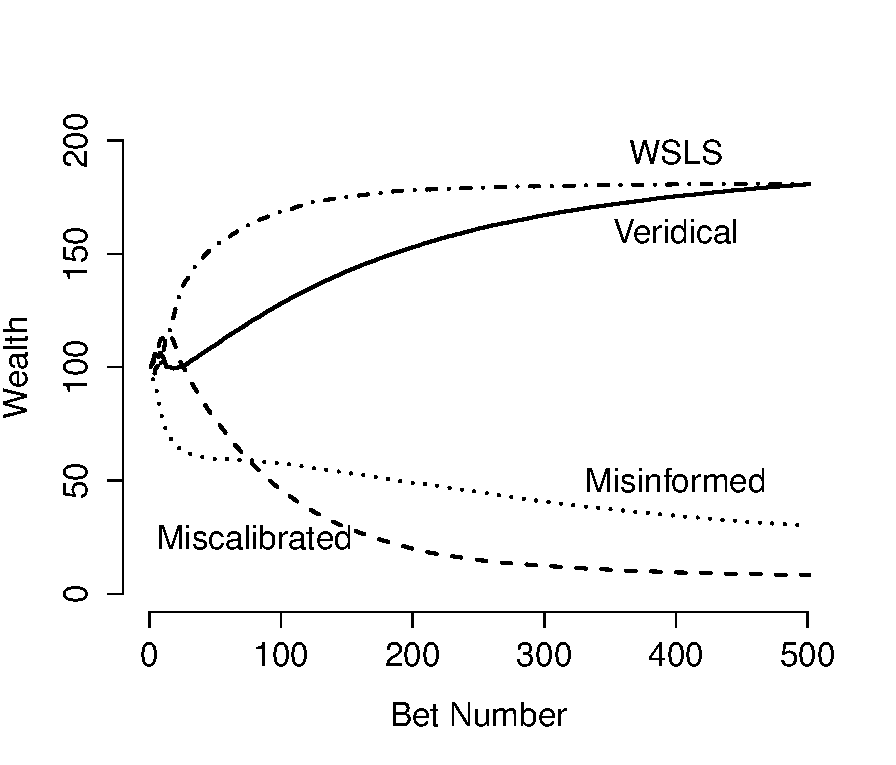
\includegraphics[width=.6\textwidth]{other_figs/threeBayesPlusWSLS.pdf}
	\caption{The gambling game from Figure~\protect\ref{fig:threeBayes} revisited, with a fourth non-Bayesian agent added to the mix. Despite its reliance on a simple win-stay lose-shift heuristic, the non-Bayesian agent is arguably the best gambler of the four. }
	\label{fig:gamblingRevisited}
\end{figure}

The conclusions from the simulations in Figure~\ref{fig:gamblingRevisited} mirror those from the original analysis---a Bayesian learner who solves the wrong problem has precious little guarantee of success in real life, and Dutch book arguments are a cold comfort to the exploited Bayesian---but extends it to highlight the fact that it is not at all easy to work out what the right problem should be. The correct solution to a {\it prediction} problem need not be the same as the solution to the corresponding {\it gambling} problem because the social environment is different. When making predictions one is not necessarily in competition with other agents, but gambling typically does put one in conflict with other people, and as a consequence the relative importance of social reasoning shifts quite dramatically. Labeling the veridical Bayesian model as ``optimal'' seems reasonable for a prediction task, but the same model is decidedly non-optimal at gambling. Of course, there is probably a Bayesian model that is ideal for the gambling problem---one that integrates social reasoning with objective learning in  a natural fashion---and we expect that this model would outperform all four of our existing models. However, this is beside the point. Our point here is that it is surprisingly easy to accidentally solve the wrong problem, and as a consequence we find ourselves very cautious about making optimality claims. 

\subsection*{Combining Bayesian data analysis with Bayesian cognition}

Although not the main focus of our discussion, one theme that has run through some of our analysis is that it is useful to combine Bayesian models of human cognition with Bayesian data analysis tools---an approach that has been appropriately dubbed {\it doubly Bayesian} \cite{Huszar2010,Hemmer2014}. For example, in order to estimate individual subject response curves in case study 1 we implemented the  Bayesian cognitive model as a parameterized model in JAGS \cite{plummer_jags:_2003}, and the curves reported in Figure~\ref{fig:indiv} were constructed by plotting the model predictions at the posterior mean parameters. This is a fairly standard way of estimating model parameters within the Bayesian data analysis tradition \cite<e.g.,>{lee_bayesian_2014}. For the most part we have moved technical details to the Appendices, in order to make the main text more readable, but it is worth noting that much of what we are able to achieve in this paper has been because we relied on principled tools for model fitting and model selection, which the Bayesian data analysis approach provides. 

The merits of combining a descriptive Bayesian cognitive model with a Bayesian data analysis are considerable. In principle, sophisticated data analysis methods are not necessary when building an optimal Bayesian model because there are no free parameters to be estimated---at least in theory if not so much in practice. The model is the very ideal of a scientific hypothesis because every relevant detail is specified a priori. This is a caricature of how optimal Bayesian models are constructed in the real world, but the issue of properly accounting for model complexity seems more important in situations where the researcher acknowledges that he or she does not know what priors or likelihoods the participant used. 

In theory, Bayesian data analysis is naturally applicable to Bayesian cognitive models: The researcher expresses their uncertainty about the participant in the form of a {\it researcher prior}, and uses the Bayesian cognitive model to express the {\it researcher likelihood}. All inferences about individual participants and all model comparisons are then based on the {\it researcher posterior} beliefs about what actually happened in the experient. This is precisely the approach to data analysis advocated elsewhere in the methodological literature \cite<e.g.,>{lee_bayesian_2014,lee_three_2008,wagenmakers_practical_2007,kruschke_doing_2010}, but we concede that it poses a uniquely awkward problem when applied to Bayesian cognitive models: The same few words (``priors'', ``likelihoods'', ``posteriors'', etc) become severely overloaded. Authors must go to considerable rhetorical lengths to disambiguate between {\it participant priors} (what subjects believe about the world) and {\it researcher priors} (what the modeler believes about the subjects). Similarly, a {\it participant likelihood} would refer to the theory that underpins a participant's learning in the experiment, whereas the {\it researcher likelihood} refers to the researcher's theory about how participants were producing responses, and thus corresponds to the entirety of the Bayesian cognitive model. A good deal of care is required to clearly disambiguate between these different entities. Even so, our view is that the power of the Bayesian data analysis framework makes it worth the effort.


\subsection*{Conclusions}

Our goals in this paper are twofold. Most importantly, we argue that researchers need to make a clear distinction between Bayesian models that make normative claims and Bayesian models that make only descriptive claims. We feel that much of the confusion in the existing literature arises because people do not make this distinction as clearly as they should. As a secondary goal---because many researchers are unsure whether Bayesian models are useful when normative claims are not made---we have sought to highlight some of the types of questions and analyses that are possible while only making descriptive claims. Descriptive Bayesian models are more modest, because they require the researcher to express ignorance about which participant priors and participant likelihoods are involved. But it is exactly this modesty that makes them more generally useful, because the expression of researcher uncertainty is what allows the model to be used as a tool to guide our learning as psychologists. Instead of having to state {\it a priori} what knowledge people {\it should} have (priors) or what learning rules they {\it should} use (likelihoods), we treat those quantities as the unknowns that we seek to learn about. 

Our three case studies, as simple as they are, illustrate several different ways in which descriptive Bayesian models can be used to learn about human cognition. The value of optimal models and normative descriptions have been debated elsewhere in the literature---it is arguably {\it the} central issue spanning the many papers that followed from the initial \citeA{jones_bayesian_2011} critique---but in our view the question of whether psychology needs {\it optimal} Bayesian models is very different to the question of whether {\it descriptive} Bayesian models are useful to the field. 
Even the somewhat cursory applications we have presented in this paper illustrate the usefulness of these models for addressing a wide range of psychological questions that go beyond the narrow---albeit powerful---focus of optimal Bayesian models. 

When combined with powerful statistical tools to perform inference (e.g., Bayesian data analysis, cross-validation, etc), we can use a flexible, descriptive Bayesian cognitive model to explore individual differences in prior beliefs and in the willingness to have data change those beliefs (case study 1). We can use them to learn about people's prior beliefs and how they compare to environmental statistics or to the performance of non-Bayesian heuristics (case study 2). Finally, we can develop tools that allow us to learn about the hypotheses that people rely on to guide their inferences (case study 3). Independent of the question about whether people's behavior is optimal, descriptive Bayesian models have an important role to play in helping us understand this behavior---which is, of course, one of the main goals of psychology.

 